\item Threads module
	
The Threads module was expected to at least implement these 6 functional processes:
	
\begin{enumerate}
\item submitPost:
	\begin{itemize}
		\item\textbf{Objective: } Used to submit a post to a thread by creating a child thread.
		\item\textbf{Pre-conditions: } The buzz space must be active (i.e. exist). The user submitting the post must exist and be a registered user on that buzz space. 
		\item\textbf{Post-conditions: } Either create a post and append it as a child to the current thread or return the relevant error message should something go wrong.
		\item\textbf{Testing: } Both pre-conditions are met. Although there is a function to generate threads in the Buzz system (createNewThread) it does not function as the submitPost functional requirements dictate it should. createNewThread allows for the creation of threads without neccessarily appending it as a child to a parent thread (which submitPost does not allow). Furthermore createNewThread is hard-coded with dummy info and is clearly used for simple display purposes (i.e. to show how a thread might have looked if the thread handling functions had been fully implemented). Since no proper implemenation of submitPost is present in the Buzz system it therefore fails the post-conditions.

\begin{figure}[h!]
  \centering
    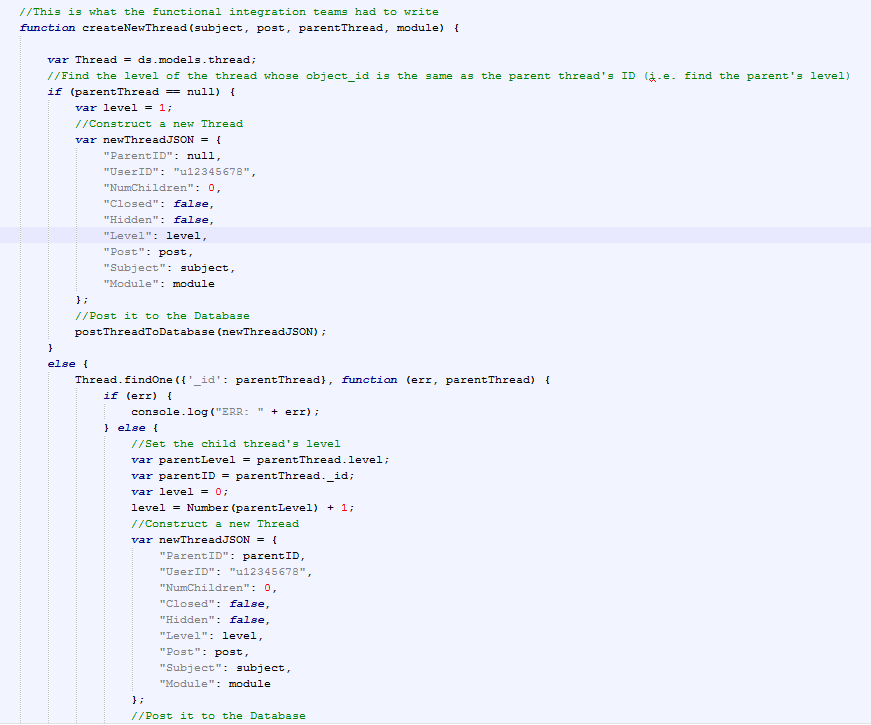
\includegraphics[width=0.85\textwidth]{createNewThread}
    \caption{Implementation of the createNewThread function}
	\end{itemize}
\item markPostAsRead:
	\begin{itemize}
		\item\textbf{Objective: } Create a data object when a user reads a post. The data object will contain information about the reading event such as which user read the post at what time.
		\item\textbf{Pre-conditions: } This function requires a post and a user to read the post so that it can save the relevant information regarding the reading event.
		\item\textbf{Post-conditions: } A data object containing information about the reading event is stored or an error message is returned.
		\item\textbf{Testing: } All pre-conditions are met but there is no function in the buzz system which implements this functional requirement, it therefore fails the post-conditions.
	\end{itemize}
\item closeThread:
	\begin{itemize}
		\item\textbf{Objective: }This closes a thread and prevents it from being further manipulated by the user. It also gives the user to either manually or autonomously summarise the thread.
		\item\textbf{Pre-conditions: } A thread to close and a user which has administrator privlidges.
		\item\textbf{Post-conditions: } The thread is closed and made inaccessible  to general users. If the summariser is implemented then a summary is made.
		\item\textbf{Testing: } All pre-conditions are met but there is no function in the buzz system which implements this functional requirement, it therefore fails the post-conditions.
	\end{itemize}
\item moveThread:
	\begin{itemize}
		\item\textbf{Objective: }  Be able to detach a sub-tree of threads from one thread and add it to another.
		\item\textbf{Pre-conditions: } A minimum of two threads (one to move and one from which it can be detached or attached to).
		\item\textbf{Post-conditions: }The threads sub-tree is either successfully moved or an error message is displayed.
		\item\textbf{Testing: } All pre-conditions are met but there is no function in the buzz system which implements this functional requirement, it therefore fails the post-conditions.
	\end{itemize}
\item hideThread:
	\begin{itemize}
		\item\textbf{Objective: } This is used to mark a thread as hidden. Hidden threads (and all their child threads) should be made inaccessible  to the users and should not be rendered by the user interface.
		\item\textbf{Pre-conditions: } This simply requires a thread to mark as hidden (a user is not required as this function is not directly accessed by users).
		\item\textbf{Post-conditions: }The thread (and all its descendants) are marked as hidden and are not displayed on the user's interface.
		\item\textbf{Testing: }  All pre-conditions are met but there is no function in the buzz system which implements this functional requirement, it therefore fails the post-conditions.
	\end{itemize}
\item queryThread:
	\begin{itemize}
		\item\textbf{Objective: } This function should return subsets of posts  according to a range of user restrictions.
		\item\textbf{Pre-conditions: }  This function requires  the user to specify the following restrictions for their query: startDateTime (return posts after this dateTime), endDateTime (return posts before this dateTime), maxLevel (return posts which are, at most, at this depth relative to the current post), minLevel(return posts which are, at least, at this depth relative to the current post), userGroup (only return posts which were posted by these specific users) and phraseSet (only return posts which contain all of these phrases).
		\item\textbf{Post-conditions: }The query should return specific information of all the posts which conform to the user specified restrictions. The information to be returned include: ParentID, Author, TimeStamp, Content and Status (e.g. closed or hidden).
		\item\textbf{Testing: } All pre-conditions are met but there is no function in the buzz system which implements this functional requirement, it therefore fails the post-conditions
	\end{itemize}
\end{enumerate}
